\documentclass{article}
\usepackage[utf8]{inputenc}
\usepackage[margin=0.8in]{geometry}
\usepackage{graphicx}
\usepackage{pgffor}
\usepackage{caption}
\usepackage{paracol}
\usepackage{chngcntr}
\usepackage{amsmath}
\usepackage{biblatex}


\addbibresource{references.bib}

\renewcommand{\b}[1]{\mathbf{#1}}
\newcommand{\singleWidth}{0.6\textwidth}

\captionsetup[figure]{
    font=small,           % Makes text smaller (can use 'footnotesize' for even smaller)
    labelfont=bf,         % Makes "Figure X" bold
    margin=10pt,          % Indents caption from the left/right of the column
    skip=5pt,             % Reduces space between image and caption
    justification=centering % Keeps it neat
}


\title{Assignment 4 Report}
\author{Group 17: \\ Darlington Nkrumah (202492437) \\
  Greg de Souza (202582225) \\
  Xuan Toan Doan (202583882)}
\date{March 2026}

\begin{document}

\maketitle

\section*{Introduction}

For assignment four, we were provided with a dataset with $14$ features to make a
random tree based classifier to identify the positive class in the Alzheimer's diagnosis. For ease
for notation, we'll refer to this 14 features as $x_i$ with $i=0,1,2,...,13$. Notably, we are counting
from zero (0) as python indexes the features.

  \section*{Question 1: Decision Tree classifier}
  
  A single decision tree classifier was trained using the provided training dataset,
  with 202 members of the negative class, and 202 members of the positive class. For
  the training procedure, we use the \textit{scikit-learn} \textit{DecisionTreeClassifier} with the
  default settings, and seeded random state. Using cross validation for model selection with 10 folds,
  we selected the best possible leaf criterion from three possible choices: \textit{gini},
  \textit{entropy} and \textit{log loss}. The candidate models were evaluated based on balanced accuracy,
  and they all achieved similar results, with the \textit{gini} feature criterion scoring $0.5296$ in
  balanced accuracy, and the two other feature criterion achieving $0.5345$, outperforming gini.
  Entropy and Log Loss achieving identical results makes sense, since the two criterion are identical
  except for a multiplicative constant. 

  The best performing criterion chosen for retraining was \textbf{entropy}. The final model was assessed
  using the test dataset provided, with 361 members of the negative class
  and 194 members of the positive class. The final assessment results are shown in table
  \ref{tab:Err}.
  Notably, the balanced accuracy on the independent test set was BETTER than expected given
  the cross validation evaluation,
  suggesting that training on additional data was very beneficial for this model.
  
  
  \section*{Question 2: Final Decision Tree}

  The final decision tree from Question 1 was plotted in figure \ref{fig:Q2_tree}, with a zoom on the root
  provided in figure \ref{fig:zoom}. As we can see from the first ``split'', the most important feature
  to differentiate the two classes is the third featured (indexed as $x_2$ when counting from zero).

  \begin{figure}[h!]
    \centering
    \includegraphics[width=0.2\textwidth]{tree_zoom.png} 
    \caption{Zoom on the root of the tree}
    \label{fig:zoom}
  \end{figure}

  
  
  \begin{figure}[htb]
    \centering
    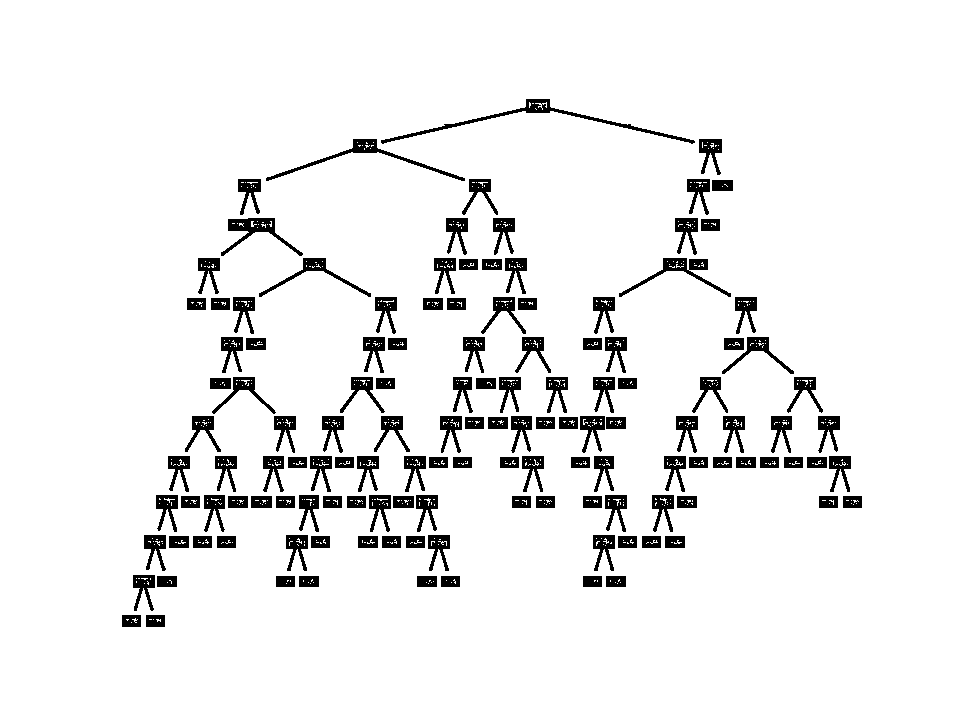
\includegraphics[width=1.0\textwidth]{Q2_tree.pdf} 
    \caption{Final decision tree for a Decision Tree Classifier with entropy as the feature criteria}
    \label{fig:Q2_tree}
  \end{figure}



  \section*{Question 3: Random Forest Classifier}
  For question 3, we now trained a Random Forest Classifier instead of a single decision tree.
  The training an testing process
  was identical to question 1, where we evaluated 3 possible feature criteria with a cross validation approach.
  For the random forest, the best feature criteria was \textbf{gini}, achieving a balanced accuracy of
  0.6826 in the cross validation, versus a balanced accuracy of 0.6782 for both \textit{log loss} and
  \textit{entropy}.

  The final model was retraining on the full training dataset using gini as a feature criteria, and assessed
  on the testing dataset provided, the results are presented in table \ref{tab:Err}. Notably, the
  Random Forest Classifier outperformed the decision tree in all metrics except Specificity, that is
  the ability to identify true negative events in the dataset.

  The overall improvement in performance was expected, as the main drawback of the single decision tree
  is that it's prone to over fitting  due to high variance, it ``follows'' the noise as well as the data.
  The random forest classifier deploys techniques like bagging and boosting to produce multiple trees
  with different leafs and features taken into account, and then averages their prediction. This process
  significantly reduces variance, making it so the classifier classifies the data, and not the noise.
  

  \begin{table}[]
    \begin{tabular}{l|l|l}
      \textbf{Err}      & \textbf{Decision Tree} & \textbf{Random Forest} \\ \hline
      Accuracy          & 0.5856                 & \textbf{0.6450}        \\
      Balanced Accuracy & 0.5920                 & \textbf{0.6771}        \\
      Sensitivity       & 0.6134                 & \textbf{0.7835}        \\
      Specificity       & 0.5706                 & 0.5706                 \\
      Precision         & 0.4343                 & \textbf{0.4951}        \\
      Recall            & 0.6134                 & \textbf{0.7835}       
    \end{tabular}
    \caption{Model assessment results for the Decision Tree and the Random Forest Classifier, based on testing data with 361 members of the negative and 194 members of the positive class.}
    \label{tab:Err}
  \end{table}

  
\end{document}
